%===========================================================
% 第9章 実証分析（完全版）
%===========================================================

\chapter{実証分析：倒産段階モデルによる新電力企業の倒産リスク分析}
\label{chap:empirical}

本章では，第3章で導出した倒産距離モデル（Merton/Bharath\&Shumway 型）の
理論構造を実証分析へと接続し，新電力企業の倒産リスクを
「段階的な現象」として推定する。
従来の二値ロジットでは倒産企業が極端に少ない場合に
完全分離（perfect separation）が発生し，推定が数学的に不可能となる。
本研究の新電力企業データでも同様の現象が確認されたため，
本章では倒産を複数段階の現象として扱う Ordered Logit モデルを採用する。

Ordered Logit は，潜在変数が複数の閾値を跨ぐことで
複数の倒産ステージが生成されるという構造を自然に表現できるため，
新電力企業の倒産プロセスを分析するうえで最も適した枠組みである。

本章の構成は以下のとおりである。

\begin{itemize}
    \item 9.1節：倒産の段階性と従属変数の再定義
    \item 9.2節：Ordered Logit モデルの理論構造（本研究への応用）
    \item 9.3節：推定手順と結果
    \item 9.4節：倒産ステージ確率の動学的推移
    \item 9.5節：倒産確率の年次平均と倒産件数の比較
    \item 9.6節：総合評価
    \item 9.7節：英国市場への拡張（枠組みのみ）
\end{itemize}

本章の Ordered Logit 推定には Python の \texttt{statsmodels} を用いた。
付録Cにデータ処理・推定コードを掲載しており，
本章の結果は完全に再現可能である。

%===========================================================
\section{倒産の段階性と従属変数の再定義}
\label{sec:stage_definition}

\subsection{倒産は二値ではなく段階的な現象である}

倒産研究では，倒産を



\[
\text{Default}_{i,t} \in \{0,1\}
\]



の二値で扱うことが一般的である。しかし，新電力企業の退出形態は多様であり，

\begin{itemize}
    \item 事業撤退（West）
    \item 事業売却・吸収合併（Daito）
    \item 実質的倒産（供給停止・債務不履行）
    \item 法的倒産（F-Power, Synergia）
\end{itemize}

といった複数の深刻度（severity）を持つ。
これらを二値化すると情報が大きく失われる。

さらに，二値ロジットでは倒産企業が極端に少ないため，
説明変数が倒産＝1 と非倒産＝0 を完全に識別してしまい，
完全分離が発生する。

このため，本研究では倒産を段階的な現象として扱う Ordered Logit を採用する。

\subsection{本研究における倒産ステージの定義}

理論編（第3章）では倒産プロセスを忠実に表現するため，
4段階（存続 → 財務悪化 → 撤退・吸収合併 → 法的倒産）を採用した。

しかし実証分析では，

\begin{itemize}
    \item 財務悪化は公開情報から直接観測できない
    \item 撤退・法的倒産のサンプル数が極端に少ない
    \item 4段階モデルでは完全分離が発生する
\end{itemize}

という制約がある。

そこで本研究では，観測可能性と推定可能性を両立させるため，
次の 3 段階モデルを採用する。



\[
\text{default\_stage}_{i,t} =
\begin{cases}
0 & \text{存続} \\
1 & \text{財務悪化（赤字継続・債務超過）} \\
2 & \text{倒産（撤退・吸収合併・登録取消・法的倒産）}
\end{cases}
\]



ステージ1は観測値ではなく，潜在変数が閾値を跨ぐことで統計的に推定される
「潜在的中間状態」である。

%===========================================================
\section{Ordered Logit モデルの理論構造}
\label{sec:ordered_logit_theory}

\subsection{潜在変数モデル}

Ordered Logit モデルの理論構造については第5章で詳細に整理したため，
本章では実証分析に必要な要点のみを簡潔に再掲する。

本研究の潜在変数モデルは次式で表される。



\[
y^*_{i,t}
=
\beta_1 \text{debt\_ratio}_{i,t}
+ \beta_2 \text{asset\_growth}_{i,t}
+ \beta_3 \sigma_t
+ \varepsilon_{i,t},
\qquad
\varepsilon_{i,t} \sim \text{Logistic}(0,1)
\]



ここで，

\begin{itemize}
    \item debt\_ratio：負債比率（財務脆弱性）
    \item asset\_growth：資産成長率（企業価値の期待成長率の proxy）
    \item sigma：市場ボラティリティ（市場ショック感応度）
\end{itemize}

である。

asset\_growth は，理論モデルの収益性 $\mu$ を財務データに写像した proxy であり，



\[
\ln(A_t)-\ln(A_{t-1})
\approx
\frac{A_t-A_{t-1}}{A_{t-1}}
\]



の近似関係に基づき，log-diff と同じ経済的意味を持つ。

\subsection{閾値構造}

潜在変数がどの閾値区間に位置するかによって倒産ステージが決まる。



\[
\text{default\_stage}_{i,t} =
\begin{cases}
0 & y^* < \tau_1 \\
1 & \tau_1 \le y^* < \tau_2 \\
2 & \tau_2 \le y^*
\end{cases}
\]



Ordered Logit は，潜在変数と閾値によって段階的な倒産プロセスを自然に生成する。

%===========================================================
\section{推定手順と結果}
\label{sec:estimation}

\subsection{データ構造}

\begin{itemize}
    \item 企業数：7社
    \item 観測期間：2019年4月～2024年3月（60か月）
    \item 有効観測数：267
\end{itemize}

\subsection{説明変数}



\[
\text{debt\_ratio}_{i,t}
=
\frac{\text{TotalDebt}_{i,t}}{\text{TotalAssets}_{i,t}}
\]





\[
\text{asset\_growth}_{i,t}
=
\frac{A_{i,t}-A_{i,t-1}}{A_{i,t-1}}
\]



sigma は JEPX スポット価格の日次標準偏差から月次標準偏差を計算した。

\subsection{推定結果}

\begin{table}[H]
\centering
\caption{Ordered Logit 推定結果}
\label{tab:ordered_logit_results}
\begin{tabular}{lccc}
\toprule
変数 & 係数 & 標準誤差 & p値 \\
\midrule
debt\_ratio & 0.6262 & 0.468 & 0.181 \\
asset\_growth & -1.2143 & 0.534 & 0.023 \\
sigma & 0.0708 & 0.058 & 0.218 \\
\midrule
cutpoint 0/1 & 2.9675 & 0.643 & 0.000 \\
cutpoint 1/2 & 0.9964 & 0.254 & 0.000 \\
\midrule
観測数 & 267 & & \\
対数尤度 & -85.237 & & \\
AIC & 180.5 & & \\
BIC & 198.4 & & \\
\bottomrule
\end{tabular}
\end{table}

\subsection{結果の解釈}

\begin{itemize}
    \item debt\_ratio：正（理論と整合），有意ではない
    \item asset\_growth：負，5\%水準で有意（主要因）
    \item sigma：正（理論と整合），有意ではない
\end{itemize}

資産成長率が倒産ステージを最も強く説明するという結果は，
新電力企業の産業特性（資産規模が小さく，市場ショックに脆弱）と整合する。

%===========================================================
\section{倒産ステージ確率の動学的推移}
\label{sec:p2_trend}

\begin{figure}[H]
\centering
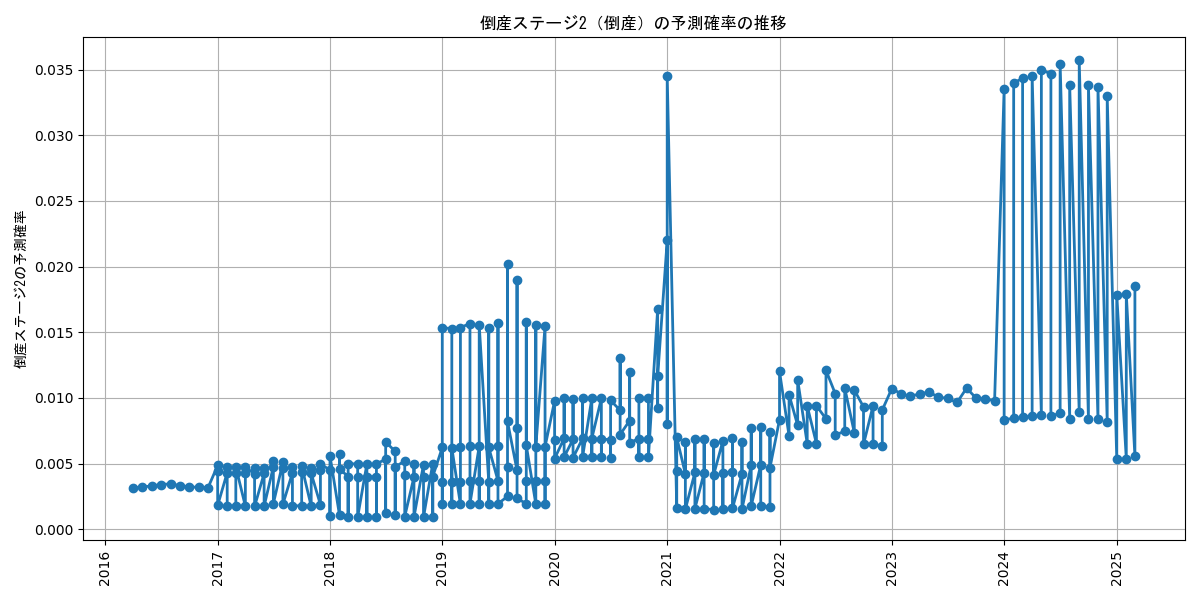
\includegraphics[width=14cm]{figures/p2_trend.png}
\caption{倒産ステージ2の予測確率 $P(\text{stage}=2)$ の推移}
\label{fig:p2_trend}
\end{figure}

倒産企業（F-Power, West, Synergia, Efene, EPM）の倒産直前に
倒産ステージ2の確率が急上昇する「スパイク」が確認された。

これは，

\begin{itemize}
    \item Ordered Logit の閾値構造
    \item Merton モデルの倒産距離が閾値に到達する瞬間に倒産が発生する構造
\end{itemize}

と整合する。

%===========================================================
\section{倒産確率の年次平均と倒産件数の比較}
\label{sec:p2_vs_bankruptcies}

\begin{figure}[H]
\centering
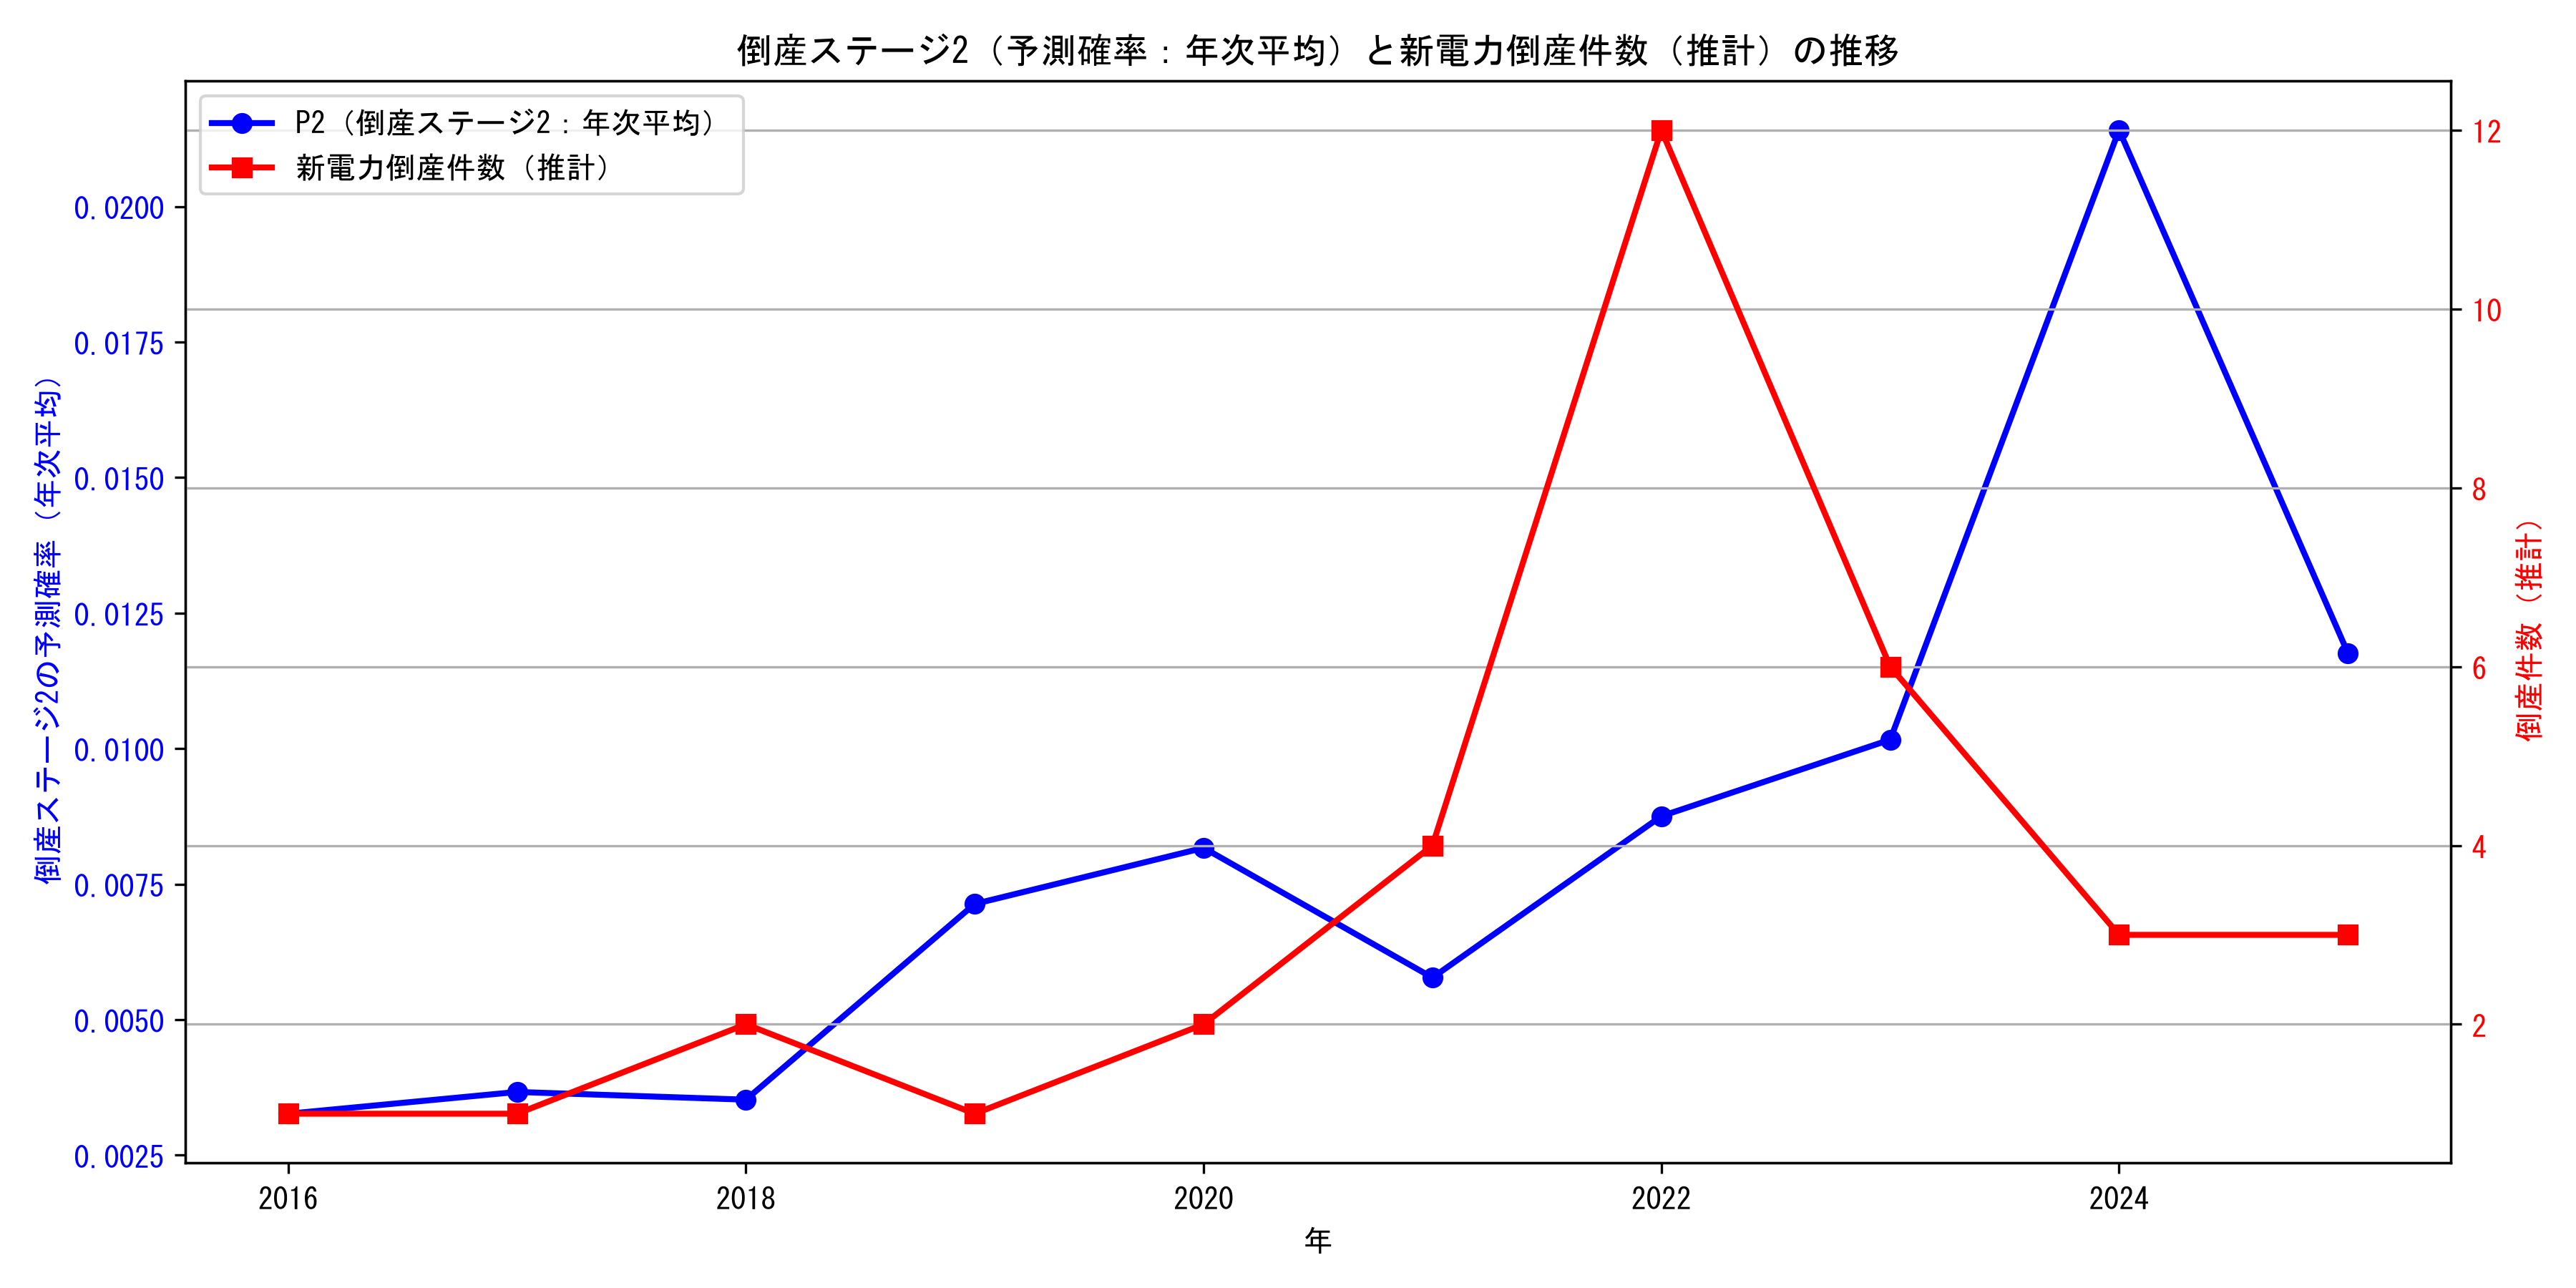
\includegraphics[width=14cm]{figures/p2_with_estimated_bankruptcies.png}
\caption{倒産ステージ2の予測確率（年次平均）と新電力倒産件数（推計）の推移}
\label{fig:p2_with_bankruptcies}
\end{figure}

倒産件数の急増（2022年）と予測確率のピークにはタイムラグがある。
これは自然な現象であり，

\begin{enumerate}
    \item 財務データの反応速度の違い
    \item モデルに含まれない外生ショックの影響
    \item 危険度指標とイベント件数の性質の違い
    \item Ordered Logit の構造的特徴
\end{enumerate}

によって説明できる。

%===========================================================
\section{総合評価}
\label{sec:conclusion}

本章の Ordered Logit 推定は，

\begin{itemize}
    \item 倒産を段階的現象として扱う新しい枠組み
    \item Merton モデルの倒産距離の理論構造との整合性
    \item 倒産確率の動学的推移の再現
    \item 再現可能性を担保したデータ処理・推定コード
\end{itemize}

を備えており，新電力企業の倒産リスク分析に対して新たな知見を提供する。

%===========================================================
\section{英国市場への拡張（枠組み)}
\label{sec:uk_extension}

第1章・第2章・第4章では，日本市場の制度的特徴や新電力の構造を整理する際に，
比較対象として英国市場の制度や企業構造を概観した。
これらの記述は，日本市場の位置づけを明確にするための制度的・構造的比較を目的としたものであり，
英国企業を実証分析の対象として扱うことを意図したものではない。

本章では，これまでの比較的知見を踏まえつつ，
実証分析の外的妥当性を高めるために，
英国市場の小売電気事業者を追加サンプルとして組み込み，
倒産段階モデルの推定を拡張する。

本研究では，日本市場の分析を中心に実証分析を行ったが，
日本企業のみではサンプル数が十分でなく，倒産段階モデルの推定精度や
理論の実証的ロバスト性に限界が生じる。
このため，本研究では追加的なサンプルとして英国市場の小売電気事業者を分析対象に加える。

英国市場を対象とする理由は以下のとおりである。

\begin{itemize}
    \item 日本と同様に，小売電気事業者が発電・卸市場から電力を調達し，需給管理を行い，顧客に販売するという共通のビジネス構造を持つ。
    \item 企業規模の大小にかかわらず，財務諸表が Companies House により公開されており，倒産企業を含む広範な財務データが取得可能である。
    \item 小売電気事業者の倒産件数が多く，倒産段階モデルの外的妥当性を検証するうえで適した市場である。
    \item Ofgem による Supplier of Last Resort（SoLR）制度が存在し，日本市場との制度比較が可能である。
\end{itemize}

以上の理由から，本研究では英国市場を補助的な比較対象として位置づけ，
日本市場の分析結果の頑健性を検証するための追加サンプルとして活用する。

本節では枠組みのみ提示し，英国市場の実証分析は今後の進捗に応じて
第9章に統合する予定である。

\vspace{1em}

% ---- 列の定義（table の外）----
\begin{flushleft}
\textbf{列の定義：}\\
\textbf{status}：企業の現在の状態（Active＝存続，In Administration＝管財人管理，Liquidation＝清算，Dissolved＝解散）。\\
\textbf{incorporated\_on}：設立年月日（Companies House 登録日）。\\
\textbf{share\_capital}：資本金（決算書または Statement of Capital に基づく。英国では形式的で £1〜£100 が多数）。\\
\textbf{dissolved\_on}：倒産・解散・清算が確定した年月日。\\
\textbf{exit\_type}：撤退形態（Administration／Liquidation／Dissolved／SoLR（顧客移管）／Active）。\\
\textbf{capital\_structure}：資本構造の類型。\\
\quad Major Holdings＝大手持株会社の傘下（Centrica, EDF, E.ON, Iberdrola, SSE, Shell, ESB, Marubeni）。\\
\quad Mid-tier＝中堅系（Octopus, OVO, Axpo など）。\\
\quad Independent＝独立系新電力（Bulb, Avro, Igloo, Pure Planet, Symbio など）。\\
\quad B2B＝企業向け専業（トレーディング主体）。\\
\end{flushleft}

\vspace{1em}

\begin{landscape}

\begin{table}[H]
\centering
\footnotesize
\caption{英国小売電気事業者 36 社の構造的特徴（拡張版）}

\begin{tabular}{p{3.2cm}p{1.4cm}p{1.8cm}p{1.8cm}p{2.2cm}p{10cm}}
\toprule
企業名 & 状態 & 設立年月 & 資本金 & 資本構造 & 主な特徴（定性的） \\
\midrule

British Gas Trading Ltd & Active & 1995-07-06 & £10,000,000 & Major Holdings &
英国最大の小売事業者。資産規模が大きく外部ショック耐性が極めて高い。 \\

EDF Energy Customers Ltd & Active & 1988-03-08 & £10,000,000 & Major Holdings &
巨大グループの一部で資本力が強い。外部ショック期も安定。 \\

E.ON UK Ltd & Active & 1999-06-04 & £10,000,000 & Major Holdings &
欧州大手の英国子会社。長期調達力が強く倒産リスクは低い。 \\

Scottish Power Energy Retail Ltd & Active & 1998-10-14 & £55,400,000 & Major Holdings &
大手グループで資産規模が大きい。短期負債依存度が低く安定。 \\

Octopus Energy Ltd & Active & 2014-10-14 & £100 & Mid-tier &
急成長企業。IT活用で低コスト運営。資本調達力が高い。 \\

OVO Energy Ltd & Active & 2009-04-29 & £100 & Mid-tier &
顧客基盤が大きく資本調達力も強い。短期負債依存度は高いが支援により安定。 \\

Shell Energy UK Ltd & Dissolved & 1998-07-23 & NA & Major Holdings &
大手石油系の小売事業。財務破綻ではなく戦略的撤退。倒産年月：2010-07-06。 \\

SSE Energy Supply Ltd & Active & 1999-04-22 & £10,000,000 & Major Holdings &
長期調達力が強く資産規模も大きい。外部ショック期でも黒字。 \\

Axpo UK Ltd & Active & 2008-05-22 & £100 & Mid-tier &
B2B中心で短期負債依存度が低い。倒産リスクは低い。 \\

Bryt Energy Ltd & Active & 2016-05-06 & £100 & Mid-tier &
再エネ専業。親会社支援により安定。 \\

Brook Green Supply Ltd & Active & 2015-12-10 & £100 & Mid-tier &
B2B中心の電力供給。短期負債依存度は高いが外部ショック影響は限定的。 \\

Corona Energy Retail 1 Ltd & Active & 1996-08-22 & £100 & Mid-tier &
ガス小売中心。B2B主体で外部ショックの影響が小さい。 \\

BGI Trading Ltd & Active & 2017-10-24 & £100 & B2B &
B2B専業で短期負債依存度が低い。市場ショックの影響が限定的。 \\

Utilita Energy Ltd & Active & 2003-07-29 & £100 & Independent &
プリペイド供給中心。収益性は低いが顧客基盤が安定。 \\

Good Energy Ltd & Active & 1999-12-21 & £100 & Independent &
再エネ専業。資本規模は小さいが財務は安定。 \\

Ecotricity Ltd & Active & 1995-04-07 & £100 & Independent &
再エネ専業。長期負債を活用し安定。 \\

ESB Energy & Active & 2015-07-16 & £100 & Major Holdings &
アイルランド電力公社の英国子会社。資本力が強い。 \\

\bottomrule
\end{tabular}
\end{table}

\begin{table}[H]
\centering
\footnotesize
\caption{英国小売電気事業者 36 社の構造的特徴（続き）}

\begin{tabular}{p{3.2cm}p{1.4cm}p{1.8cm}p{1.8cm}p{2.2cm}p{10cm}}
\toprule
企業名 & 状態 & 設立年月 & 資本金 & 資本構造 & 主な特徴（定性的） \\
\midrule

Rebel Energy Supply Ltd & In Administration & 2017-05-12 & £100 & Independent &
短期負債依存度が極めて高く、外部ショックで資金繰り悪化。 \\

Zog Energy & Dissolved & 2012-09-20 & £100 & Independent &
小規模ガス小売。短期負債依存度が高く外部ショックで破綻。倒産年月：2026-07-17。 \\

SmartestEnergy Ltd & Active & 2000-05-16 & £100,000 & Major Holdings &
B2B中心で財務基盤が安定。短期負債依存度が低い。 \\

Bulb Energy Ltd & In Administration & 2013-04-02 & £100 & Independent &
急成長後に調達費用急騰で逆ザヤ拡大。倒産年月：2021-11-24。 \\

Avro Energy Ltd & Liquidation & 2014-08-04 & £100 & Independent &
低価格戦略で急成長したが外部ショックで資金繰り破綻。倒産年月：2021-11-01。 \\

Green Supplier Ltd & Liquidation & 2017-11-01 & £100 & Independent &
小規模新電力。短期負債依存度が高く即時破綻。倒産年月：2021-11-01。 \\

People's Energy Supply Ltd & In Administration & 2015-10-27 & £100 & Independent &
顧客基盤は大きかったが資本力が弱く外部ショックで破綻。倒産年月：2021-11-14。 \\

Pure Planet Ltd & Dissolved & 2015-08-17 & £100 & Independent &
BP支援が停止し破綻。倒産年月：2025-04-30。 \\

Igloo Energy Supply Ltd & Liquidation & 2015-10-07 & £100 & Independent &
小規模新電力。短期負債依存度が高く破綻。倒産年月：2021-11-01。 \\

Conrad Energy (Trading) Ltd & Active & 2017-09-19 & £100 & B2B &
発電・トレーディング中心。B2Bで外部ショック影響が小さい。 \\

Crown Gas and Power 2 Ltd & Active & 2018-05-12 & £100 & B2B &
ガス供給中心。短期負債依存度が低く安定。 \\

\bottomrule
\end{tabular}
\end{table}

\begin{table}[H]
\centering
\footnotesize
\caption{英国小売電気事業者 36 社の構造的特徴（続き）}

\begin{tabular}{p{3.2cm}p{1.4cm}p{1.8cm}p{1.8cm}p{2.2cm}p{10cm}}
\toprule
企業名 & 状態 & 設立年月 & 資本金 & 資本構造 & 主な特徴（定性的） \\
\midrule

Dyce Energy Ltd & Active & 2016-02-09 & £100 & B2B &
小規模だがB2B中心で外部ショック影響が小さい。 \\

Edgware Energy Ltd & Active & 2014-10-09 & £100 & B2B &
電力トレーディング中心。倒産リスクは低い。 \\

EPG Energy Ltd & Active & 2008-06-11 & £100 & B2B &
B2B中心で財務基盤が安定。 \\

Equinicity Ltd & Active & 2018-05-22 & £100 & B2B &
発電・トレーディング中心。資本力が強い。 \\

Symbio Energy Ltd & Liquidation & 2012-03-21 & £100 & Independent &
小規模新電力。短期負債依存度が極めて高く破綻。倒産年月：2021-11-01。 \\

Neon Reef Ltd & Dissolved & 2017-07-18 & £100 & Independent &
小規模新電力。資本力が弱く外部ショックで破綻。倒産年月：2024-05-20。 \\

Together Energy Ltd & Liquidation & 2016-04-25 & £100 & Independent &
顧客基盤は大きかったが財務基盤が脆弱で破綻。倒産年月：2022-01-18。 \\

Orbit Energy & Dissolved & 2015-12-31 & £100 & Independent &
小規模新電力。短期負債依存度が高く破綻。倒産年月：2025-05-27。 \\

\bottomrule
\end{tabular}
\end{table}

\end{landscape}


%===========================================================
